\begin{frame}

\begin{figure}[!tbp]
  \centering
  \begin{minipage}[b]{0.45\textwidth}
    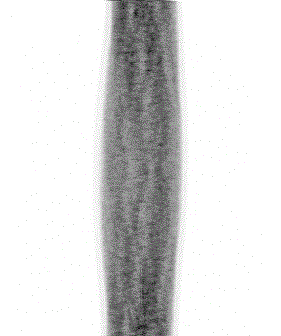
\includegraphics[width=\textwidth]{Images/sinogram_head.png}
  \end{minipage}
\pause
  \hfill
  \begin{minipage}[b]{0.45\textwidth}
    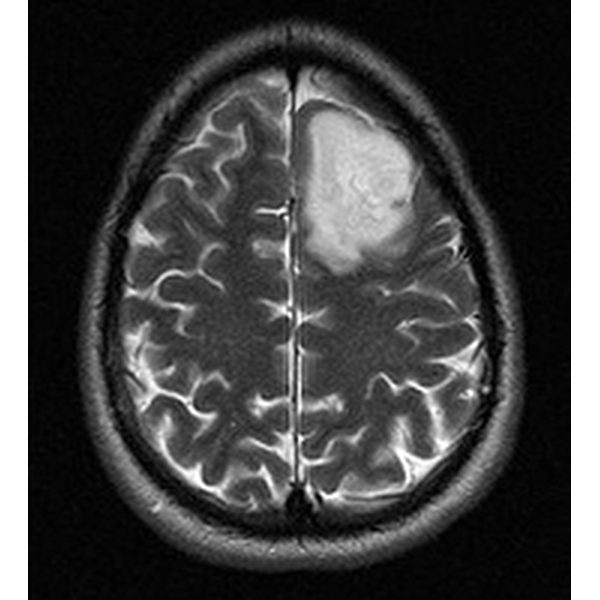
\includegraphics[width=\textwidth]{Images/brain_tumor.jpg}
  \end{minipage}
\end{figure}
\end{frame}

\begin{frame}
\begin{figure}[!tbp]
\includegraphics[width=0.9\textwidth]{Images/CT_scan.jpg}
\end{figure}
\end{frame}

\begin{frame}{CT Reconstruction}

\begin{block}{Forward model}
Given by the X-ray transform $\mathcal{R}: L^2(\mathbb{R}^2)\longrightarrow L^2(\mathbb{S}^1\times\mathbb{R})$:
$$
g = \mathcal{R}f(\theta,s)= \int_{-\infty}^{\infty}\int_{-\infty}^{\infty}f(x,y)\delta(x\cos\theta+y\sin\theta-s)dxdy
$$
where $f\in \mathcal{D}'(\mathbb{R}^2)$.
\end{block}

\pause
\bigskip

\textbf{Ill-posedness:}    
\begin{itemize}
\item Filtered back projection ($\mathcal{R}^{-1}$) involves differentiation $\longrightarrow$ increases singularities and noise.
 
\item $\mathcal{R}^{-1}$ is unbounded $\longrightarrow$ two far apart images can have very close X-ray transform.
\end{itemize}
\end{frame}


\begin{frame}{Shepp-Logan phantom}
\begin{figure}[!tbp]
  \centering
  \begin{minipage}[b]{0.45\textwidth}
    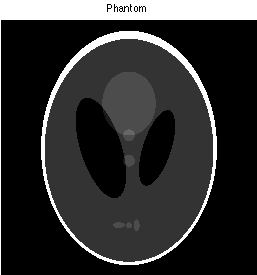
\includegraphics[width=\textwidth]{Images/phantom.png}
  \end{minipage}
  \hfill
  \begin{minipage}[b]{0.45\textwidth}
    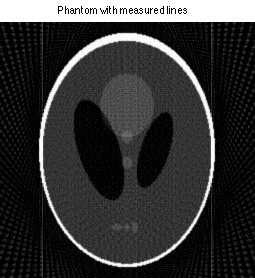
\includegraphics[width=\textwidth]{Images/phantom_measured.png}
  \end{minipage}
\end{figure}
\end{frame}

\begin{frame}{Sinogram}
\begin{figure}[!tbp]
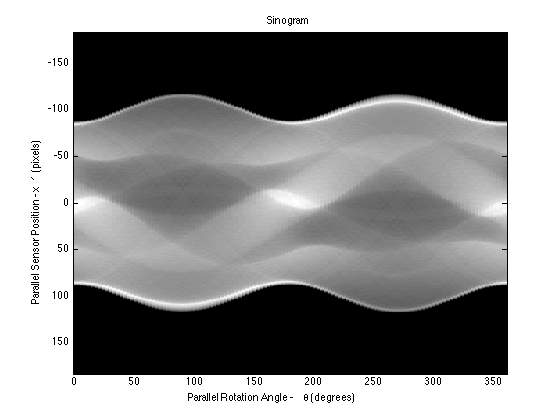
\includegraphics[width=0.9\textwidth]{../sinogram.png}
\end{figure}
\end{frame}

\begin{frame}{Solving inverse problems}
\begin{block}{First approach}
Minimizing the miss-fit against data:
$$
\min_{f} \mathcal{L}(\mathcal{R}(f),g)
$$
e.g. $\mathcal{L}(\mathcal{R}(f),g)=||\mathcal{R}(f)-g||_2^2$. \textbf{Downside:} Ill-posedness results on overfitting.
\end{block}

\bigskip
\pause

\textbf{Approaches to address overfitting?:}
\begin{itemize}
\item \textbf{Knowledge-driven regularization:} Model prescribed beforehand using first principles, data used to calibrate the model.
\item \textbf{Data-driven regularization:} Model learned from data, without any prior first principles.
\item \textbf{Hybrid:} Best of both worlds. 
\end{itemize}
\end{frame}

\begin{frame}{Knowledge-driven regularization}
\begin{block}{\textbf{Pros \Smiley{}}}
\begin{itemize}
\item Guided by first principles (laws encoded by equations), tested and validated independently.
\item Not much data required.
\item Simple concepts, aiding the understanding.
\end{itemize}
\end{block}
\pause
\begin{block}{\textbf{Cons \Frowny{}}}
\begin{itemize}
\item Requires explicit description of causal relations, not always a good model exists.
\item Hard to account uncertainty quantification.
\end{itemize}
\end{block}
\pause
\begin{itemize}
\item \textbf{Examples:} Analytic pseudoinverse (e.g. FBP), Iterative methods with early stopping (e.g. ART), Variational methods (e.g. TV, $\ell^1$). 
\end{itemize}
\end{frame}

\begin{frame}{Data-driven regularization}
\begin{block}{\textbf{Pros \Smiley{}}}
\begin{itemize}
\item Deep understanding of the problem is not needed, just a lot of data.
\item Can capture complicated causal relations without making limiting assumptions.
\end{itemize}
\end{block}

\pause

\begin{block}{\textbf{Cons \Frowny{}}}
\begin{itemize}
\item Does not provide any conceptual simplification (not much conceptual understanding is acquired).
\item Not easy to incorporate a-priori knowledge. 
\item Computationally exhaustive.
\end{itemize}
\end{block}

\pause

\begin{itemize}
\item \textbf{Basic idea:} Parametrized $\mathcal{R}^{\dagger}_{\theta}: L^2(\mathbb{S}^1\times\mathbb{R})\longrightarrow L^2(\mathbb{R}^2)$ s.t. $\mathcal{R}^{\dagger}_{\theta}(g)\approx f_{\text{true}}$ $\forall \theta\in\Theta$ whenever $\mathcal{R}(f_{\text{true}})=g$. It estimates $\theta$ minimizing a loss $L:\Theta\longrightarrow \mathbb{R}^+_{0}$.
\end{itemize}
\end{frame}

\begin{frame}{Hybrid methods}

\begin{block}{Motivation}
\begin{itemize}
\item If $\mathcal{R}$ is \textbf{local} (e.g.\ deblurring, denoising) $\longrightarrow$ CNN and sufficient known pairs $(g,f_{\text{true}})$ are enough to reconstruct (Jin et al., 2016).

\item If  $\mathcal{R}$ is \textbf{global} (e.g.\ CT, MRI) $\longrightarrow$ CNN does not work, it becomes unfeasible to work with fully connected layers.
\end{itemize}
\end{block}

\pause

\begin{block}{Possible solutions}
\begin{itemize}
\item \textbf{Learned post-processing:} First an initial (not learned) reconstruction (e.g.\ FBP), and denoise with CNN (Chen et al., 2017).
\item \textbf{Learned regularizer:} Learn a regularization functional (e.g.\ dictionary learning) and perform variational regularization (Xu et al.\, 2012).
\item \textbf{Learned iterative schemes:} Using as model a classical optimization iterative method and learn the best update in each iteration using a-priori information (\"Oktem et al.\, 2017).
\end{itemize}
\end{block}

\end{frame}

\begin{frame}{Primal-dual algorithm}
 Minimization problem:
$$
\min_{f\in L^2(\mathbb{R}^2)} \mathcal{L}(\mathcal{R}(f),g)+\mathcal{S}(f)
$$
\pause
\begin{algorithm}[H]
\begin{algorithmic}[1]
\STATE Given $\sigma, \tau>0$ s.t. $\sigma\tau||\mathcal{R}||<1$, $\gamma\in [0,1]$ and $f_0\in L^2(\mathbb{R}^2)$, $h_0\in L^2(\mathbb{S}^1\times\mathbb{R})$: 
\FOR{$i=1, \ldots, I$}
\STATE $h_{i+1}\longleftarrow \text{prox}_{\sigma\mathcal{L}} (h_i+\sigma \mathcal{R}(\overline{f}_i))$
\STATE $f_{i+1}\longleftarrow \text{prox}_{\tau \mathcal{S}}(f_i-\tau[\partial\mathcal{R}(f_i)]^*(h_{i+1}))$
\STATE $\overline{f}_{i+1}\longleftarrow f_{i+1}+\gamma (f_{i+1}-f_i)$
\ENDFOR
\end{algorithmic}
\caption{Non-linear primal-dual algorithm}
\label{alg:seq}
\end{algorithm}
\pause
\textbf{Proximal operator:}
$$
\text{prox}_{\tau \mathcal{S}}(f)=\argmin_{f'\in L^2(\mathbb{R}^2} \left[ \mathcal{S}(f')+\frac{1}{2\tau}||f'-f||^2_2\right]
$$
\end{frame}

\begin{frame}{Learned primal-dual algorithm (\"Oktem et al.\, 2017)}
\begin{algorithm}[H]
\begin{algorithmic}[1]
\STATE Given $f_0\in L^2(\mathcal{R}^2)$, $h_0\in L^2(\mathcal{S}^1\times \mathbb{R})$
\FOR{$i=1, \ldots, I$}
\STATE $h_{i+1}\longleftarrow \Gamma_{\theta_{i+1}^d} (h_i,\mathcal{R}(f_i),g)$
\STATE $f_{i+1}\longleftarrow \Lambda_{\theta_{i+1}^p} (f_i,[\partial\mathcal{R}(f_i)]^*(h_{i+1}))$
\ENDFOR
\end{algorithmic}
\caption{Learned primal-dual algorithm}
\label{alg:seq}
\end{algorithm}

\pause

\textbf{Primal and dual operators:} $\Gamma_{\theta^d}$ and $\Lambda_{\theta^p}$ are learned CNN-ResNets of the form:

$$
Id+\mathcal{W}_{w_d,b_d}\circ \mathcal{A}_{c_d}\circ\ldots\circ\mathcal{W}_{w_2,b_2}\circ\mathcal{A}_{c_2}\circ\mathcal{W}_{w_1,b_1}\circ\mathcal{A}_{c_1}
$$
where,
$$
\mathcal{W}_{w_i,b_i}(f')=b_i+w_i\ast f'
$$
$$
\mathcal{A}_{c_i}(x)=\text{PReLU}(x) = \begin{cases} x & \text{if $x\geq 0$} \\ -c_i & \text{else} \end{cases}
$$
\end{frame}

\begin{frame}{Architecture}
\begin{figure}[!tbp]
  \centering
    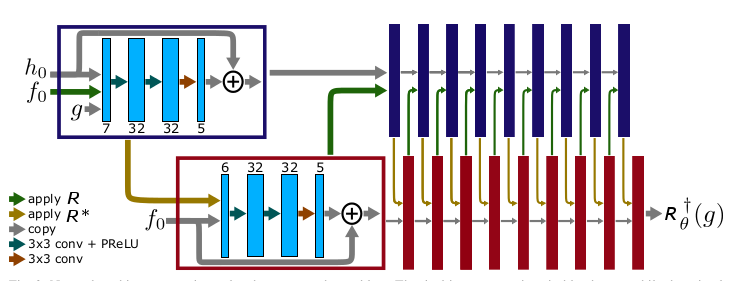
\includegraphics[width=\textwidth]{Images/architecture.png}
\end{figure}
\end{frame}

\begin{frame}{Benchmarks (Adler,\"Oktem)}
\begin{figure}[!tbp]
  \centering
    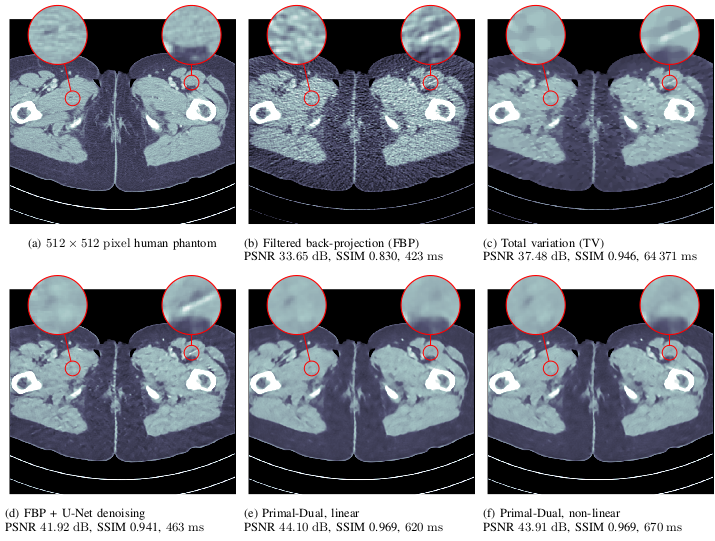
\includegraphics[width= 0.68\textwidth]{Images/lpdrec.png}
\end{figure}
\end{frame}


\begin{frame}{Wavefront set as extra information}
\begin{definition}[N-Wavefront set]
Let $N\in\mathbb{R}$ and $f$ a distribution on $\mathbb{R}^2$. We say $(x,\lambda)\in \mathbb{R}^2\times \mathbb{R}^2$ is a $N-$regular directed point if there exists a nbd.\ of $U_x$ of $x$, a smooth cutoff function $\Phi$ with $\Phi\equiv 1$ on $U_x$ and a nbd.\ $V_{\lambda}$ of $\lambda$ such that:
$$
(\Phi f)^{\wedge}(\eta)=O((1-|\eta|)^{-N}) \quad \text{for all}\quad \eta=(\eta_1,\eta_2) \quad \text{such that}\quad \frac{\eta_2}{\eta_1}\in V_{\lambda}
$$
The $N-$Wavefront set $WF^N(f)$ is the complement of the $N-$regular directed point. The Wavefront Set $WF(f)$ is defined as 

\begin{equation}
\label{eq:Wavefront-set}
WF(f)=\cup_{N>0}WF^N(f)
\end{equation}
\end{definition}

\pause
\bigskip
\begin{itemize}
\item How can we compute the wavefront set?
\item How can we incorporate it in the learned primal-dual reconstruction?
\end{itemize}
\end{frame}

\begin{frame}{Answer: Continuous Shearlet frames and Canonical relation}
\begin{block}{Classical Shearlet Transform (Guo, Kutyniok, Labate; 2006)}
$$
\langle f,\psi_{a,s,t}\rangle =\int_{\mathbb{R}^2}f(x)\overline{\psi_{a,s,t}(x)}dx
$$
where
$$
\mathcal{SH}(\psi)=\{\psi_{a,s,t}(x):=a^{-3/4}\psi (S_sA_ax-t):(a,s,t)\in \mathbb{R}_+\times\mathbb{R}\times\mathbb{R}^2\}
$$
and

$$
A_a:=
\left(
\begin{matrix}
a^1 & 0 \\
0 & a^{1/2}
\end{matrix}
\right)
\quad
S_s:=
\left(
\begin{matrix}
1 & s \\
0 & 1
\end{matrix}
\right)
$$
\end{block}
\end{frame}

\begin{frame}{Resolution of the WF set with Shearlets}

\begin{theorem}[Grohs, 2011] 
\label{thm:Resolution2}
Let $\psi$ be a Schwartz function with infinitely many vanishing moments in $x_2$-direction and $\{\psi_{a,s,t}\}$ a CSF\@. Let $f$ be a tempered distribution and $\mathcal{D}=\mathcal{D}_1\cup\mathcal{D}_2$, where

$$
\begin{aligned}
\mathcal{D}_1=\{ (t_0,s_0)\in\mathbb{R}^2\times [-1,1]|& \text{for $(s,t)$ in a neighbourhood $U$ of $(s_0,t_0)$},\\
&|\mathcal{SH}_{\psi}f(a,s,t)|=O(a^k),\forall k\in\mathbb{N} \}
\end{aligned}
$$

and

$$
\begin{aligned}
\mathcal{D}_2=\{ (t_0,s_0)\in\mathbb{R}^2\times [1,\infty)|& \text{for $(1/s,t)$ in a neighbourhood $U$ of $(s_0,t_0)$},\\
&|\mathcal{SH}_{\tilde{\psi}}f(a,s,t)|=O(a^k), \forall k\in \mathbb{N} \}
\end{aligned}
$$
Then,

$$
WF(f)=\mathcal{D}^c
$$
\end{theorem}
\end{frame}

\begin{frame}
\begin{block}{Canonical relation (\"Oktem, Quinto; 2008)}
Let $f\in D'(\mathbb{R}^2)$, and assume $\mathbb{R}(\theta,s)$ is given on an open set $U\subset [0,\pi)\times\mathbb{R}$. Let $(
\theta_0,s)\in U$, let 
$$\xi_0 = \xi_s e_s+\xi_{\sigma}\sigma(\theta_0) \perp (\cos(\theta_0),\sin(\theta_0))$$

Moreover, let  $x_0\in \ell(\theta_0,s)$. Then $(x_0,\xi_0 dx)\in WF(f)$ if and only if
$$
((\theta_0,s),(\xi_{\sigma}x\cdot\omega(\theta_0))d\theta+\xi_sds)\in WF(\mathcal{R}(f))
$$ 
\end{block}
\pause

\begin{figure}[!tbp]
  \centering
    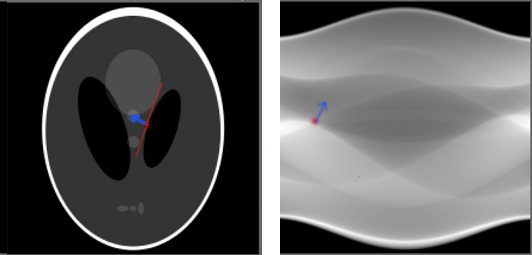
\includegraphics[width= 0.85\textwidth]{Images/CT_canonical.png}
\end{figure}
\end{frame}

\begin{frame}
\begin{block}{Shearlets on the sinogram}
\begin{itemize}
\item Let $\{\psi_{a,s,t}\}_{(a,s,t)\in\mathbb{R}^+\mathbb{R}\times\mathbb{R}^2}$ continuous compactly compactly supported shearlet, with support on $[0,2\pi)\times\mathbb{R}$, that form a frame of $L^2([0,\pi),\mathbb{R})$. 

\bigskip

Then, the system $\{\tilde{\psi}_{a,s,t}\}_{(a,s,t)\in\mathbb{R}^+\mathbb{R}\times([0,\pi)\times\mathbb{R})}$ given by

$$
\tilde{\psi}_{a,s,t}(\theta,s):=\sum_{n\in \mathbb{Z}}\psi_{a,s,t}(\theta+n\pi,s)
$$
is a Continuous Shearlet frame for $L^2(\mathbb{S}^1\times\mathbb{R})$.

\end{itemize}
\end{block}

\bigskip
\pause

\begin{itemize}
\item We have all the tools!
\end{itemize}
\end{frame}

\begin{frame}{Modified learned primal-dual}

 Modified problem:
$$
\min_{f\in L^2(\mathbb{R}^2)} \mathcal{L}(\mathcal{R}(SH_{\psi}^{-1}\tilde{f}),g) \quad \text{s.t. \textbf{C}$(WF(SH_{\psi}^{-1}\tilde{f})))$=$WF(g)$}
$$

\begin{algorithm}[H]
\begin{algorithmic}[1]
\STATE Given $\tilde{f}_0\in L^2(\mathbb{R}^2)$, $h_0\in L^2(\mathbb{S}^1\times \mathbb{R})$
\FOR{$i=1, \ldots, I$}
\STATE $h_{i+1}\longleftarrow \Gamma_{\theta_{i+1}^d} (h_i,\mathcal{R}(SH_{\psi}^{-1}\tilde{f}_i)),g)$
\STATE $\tilde{f}_{i+1}\longleftarrow \Lambda_{\theta_{i+1}^p} (f_i,[\partial\mathcal{R}(SH_{\psi}^{-1}\tilde{f_i}))]^*(h_{i+1}))$
\STATE \textbf{C}$(WF(SH_{\psi}^{-1}\tilde{f}_{i+1})))$=$WF(h_{i+1})$
\ENDFOR
\end{algorithmic}
\caption{Modified learned primal-dual algorithm}
\label{alg:seq}
\end{algorithm}

\pause
\bigskip

Are we done? \pause \textbf{Of course not!. Where is the code?!}
\end{frame}

\begin{frame}{Implementation}
\begin{itemize}
\item Learned primal dual on the Shearlet coefficients. \checked

\pause
\bigskip

\item Wavefront set computation:
\pause 

\begin{itemize}

\bigskip

\item Theory works on continuous distributions.

\pause
\bigskip

\item One needs infinite number of shearlet coefficients.

\pause
\bigskip

\item There is no faithful digital Wavefront set version (Petersen, 2018).

\pause
\bigskip

\item Learned Wavefront set extractor (in progress).
\end{itemize}

\bigskip
\pause

\item \textbf{Lesson:} Don't assume the continuous theory will work in the computer \Frowny{}.
\end{itemize}
\end{frame}

\begin{frame}{Thanks!}
\begin{center}
\Large{Questions?}
\end{center}
\end{frame}

